\section{Calculating Expected Size of the PRL}
\label{appendix:markov}

This appendix covers the basics of the utilized probabilities to then explain
the Markov matrix. We also describe the calculation of the stationary
distribution as a means to calculate the expected \ac{PRL} size. Finally, we
discuss the computation of the probabilities and expected values used in
\cref{section:eval-prl-size}.

\subsection{Utilized Probabilities}

Recall from \cref{section:eval-prl-size} that we model the processes of gaining
and losing pseudonyms from the \ac{PRL} as two individual probabilities, then we
combine them in the next step into a Markov chain. The two probabilities shown
in \cref{eq:prl-size-g} and \cref{eq:prl-size-l} are denoted as $G_{il}$ and
$L_{il}$ respectively and can be seen as probability matrices that at location
$il$ have the probability for being in state $i$ and gaining or losing $l$
pseudonyms from the list. The core assumption for these two probabilities is
that both adding and removing pseudonyms from the revocation list can be seen as
a binomial distribution that only depends on:
\begin{inparaenum}
    \item the current size of the list, i.e., how many certificates there are left to be revoked or removed from the list,
    \item the probability for each pseudonym to be revoked at any given time, and
    \item the time that a pseudonym stays in the list.
\end{inparaenum}
As such, this model assumes that pseudonyms are renewed as soon as they are
evicted from the \ac{PRL}, i.e., the list can never hold more than the total
number of $n$ pseudonyms, which is a realistic assumption for large $n$ as it is
unlikely that so many pseudonyms in the system would be revoked in a short time
during regular operation.  Furthermore, in this way we model the process of
losing pseudonyms from the list as a probabilistic process that has the expected
value at $T_{prl}$.  We, however, can not model a precise eviction of the
pseudonym from the \ac{PRL} after $T_{prl}$ time steps.  In our view this is an
acceptable tradeoff as on average and over the lifetime of the \ac{PRL}, the
modeled behavior comes very close to the actual behavior of evicting pseudonyms
from the \ac{PRL} after exactly $T_{prl}$ time steps.

\subsection{Markov Model}
We can now combine these two probabilities into a matrix that at location
$p_{ij}$ has the probability of moving from state $i$ to state $j$. Starting
with the simple example of $n=3$ pseudonyms, multiple entries of this matrix are
straightforward:
\begin{itemize}
    \item Starting at any state $i$ and stepping into state $j=0$ requires to not revoke any new pseudonyms and to lose all existing pseudonyms from the list. This is the combination of the two probabilities $L_{ii}G_{i0}$. For example, going from state $i=2$ to $j=0$ requires to lose 2 pseudonyms when there are $2$ in the \ac{PRL}, and requires to gain no new pseudonyms when there are already $2$, leading to the two probabilities $L_{22}G_{20}$
    \item Starting at state $i=0$ and stepping into a state $j$ implies that no pseudonyms can be lost from the \ac{PRL} and $j$ pseudonyms have to be added.
    \item Similarly, starting in state $i=3$ and stepping into any state $j$
    implies that no pseudonyms can be gained, but $j-i$ pseudonyms are removed
    from the \ac{PRL}.
\end{itemize}

The most interesting state transitions in this probability matrix are the
transitions that consist of multiple combinations of events. One example is the
transition from $i=2$ to $j=1$. Here, we first have the obvious possibility that
we reach the state $j=1$, i.e., one pseudonym in the \ac{PRL}, by losing one
pseudonym and gaining none. However, we also have the possibility to lose both
pseudonyms in the \ac{PRL} and gain one, leading to still one remaining
pseudonym in the \ac{PRL}. This is because the pseudonyms in the \ac{PRL} and
outside of the \ac{PRL} are independent and pseudonyms can still be revoked
while others are removed from the list. Thus, the state transition consists of
the following parts: $p_{21} = L_{21}G_{20} + L_{22}G_{21}$.

The full state probability matrix for $n=3$ pseudonyms can be seen below. Note
that a matrix for $n$ pseudonyms is a $n+1 \times n+1$ matrix to accommodate the
state of the empty \ac{PRL}.\vspace{2mm}\\
\begin{math}
    P =
    \left[ {\begin{smallmatrix}{}
      L_{00}G_{00} & L_{00}G_{01} & L_{00}G_{02} & L_{00}G_{03} \\
      L_{11}G_{10} & L_{10}G_{10} + L_{11}G_{11} & L_{10}G_{11} + L_{11}G_{12} & L_{10}G_{12} \\
      L_{22}G_{20} & L_{21}G_{20} + L_{22}G_{21} & L_{20}G_{20} + L_{21}G_{21} & L_{20}G_{21} \\
      L_{33}G_{30} & L_{32}G_{30} & L_{31}G_{30} & L_{30}G_{30} \\
    \end{smallmatrix} } \right]
\end{math}
\vspace{2mm}

\begin{figure}
    \centering
    \includegraphics[width=.85\columnwidth]{figures/markov-tikzplot/small-tikz.pdf}
    \caption{A graph of the Markov chain with the exemplary parameters of $n=3$, $p=0.1$, and $T_{prl}=2$.}
    \label{fig:appendix:markov-graph}
\end{figure}

Such probability matrices are also called discrete time Markov
chains~\cite{hermanns2002markov}. \Cref{fig:appendix:markov-graph} depicts the
transition graph for the above Markov chain when we assume the parameters of
$p=0.1$ and $T_{prl}=2$. Based on this first small example, we can approach a
closed formula for an arbitrary number of pseudonyms ($n$). This closed formula
is shown in \cref{eq:prl-size-markov}. The core idea is that each entry depends
on a combination of gaining and losing pseudonyms based on the maximum of $i-j$
and $0$ and ranges up to $i$. Then, any state combination that is not possible
will be $0$ through the binomial coefficient. However, this range is necessary
to catch the complicated combinations in the center of the matrix. Each
combination is then based on losing $l$ pseudonyms from the list and gaining
$l-i+j$ pseudonyms, which basically iterates through the combinations with $l$
as a stepping variable.

\subsection{Calculating the Expected PRL Size}

In discrete time Markov chains, a probability state vector $\pi$ can be multiplied with the Markov matrix $P$ to gain the probabilities for $\pi$ after a single transition in the model~\cite{hermanns2002markov} as follows: $\pi' = \pi \cdot P$.
This, however, is only sufficient to gain the state probabilities after specific amounts of steps.
In contrast to this approach, Markov chains may approach a so-called state equilibrium which is a stationary probability distribution that does not change even after taking a step in the Markov chain.
The stationary distribution follows the equation $\pi = \pi \cdot P$~\cite{hermanns2002markov}.

To gain this stationary distribution, we solve the following equation system:
\begin{flalign*}
                &\pi = \pi P&\\
&\leftrightarrow \pi - \pi P = 0&\\
&\leftrightarrow \pi ( I - P ) = 0&\\
&\leftrightarrow ( I - P )^T \pi^T = 0&
\end{flalign*}

Lastly, since there may be several solutions to this linear equation, we add the
specific constraint to this equation system that the sum of $\pi$ is equal to
$1$. This is the case for each probability vector in Markov
models~\cite{hermanns2002markov}, and follows the intuition that, from any state
probability, the probability to reach any other state is $1$. To add this
constraint, we add a row of $1$ to $( I - P )^T$ and append a $1$ to the zero
vector. Solving this linear equation yields a stationary distribution that is
stable. \cref{fig:eval-prl-size} summarizes this stationary distribution by
showing the list sizes that occur to 75\%, 90\%, and to 99.99\%. The graph shows
these percentiles under different scenarios, i.e., with different shares of
attackers in the network.

\begin{figure}[t]
    \centering
    \resizebox{.83\linewidth}{!}{% changed from auto generated plot:
% width=\columnwidth,
% legend pos=north west,
% and escape the % signs in the labels
% Color order: steelblue88116163 peru20313699 mediumseagreen95157109 indianred1819295
% This file was created with tikzplotlib v0.10.1.
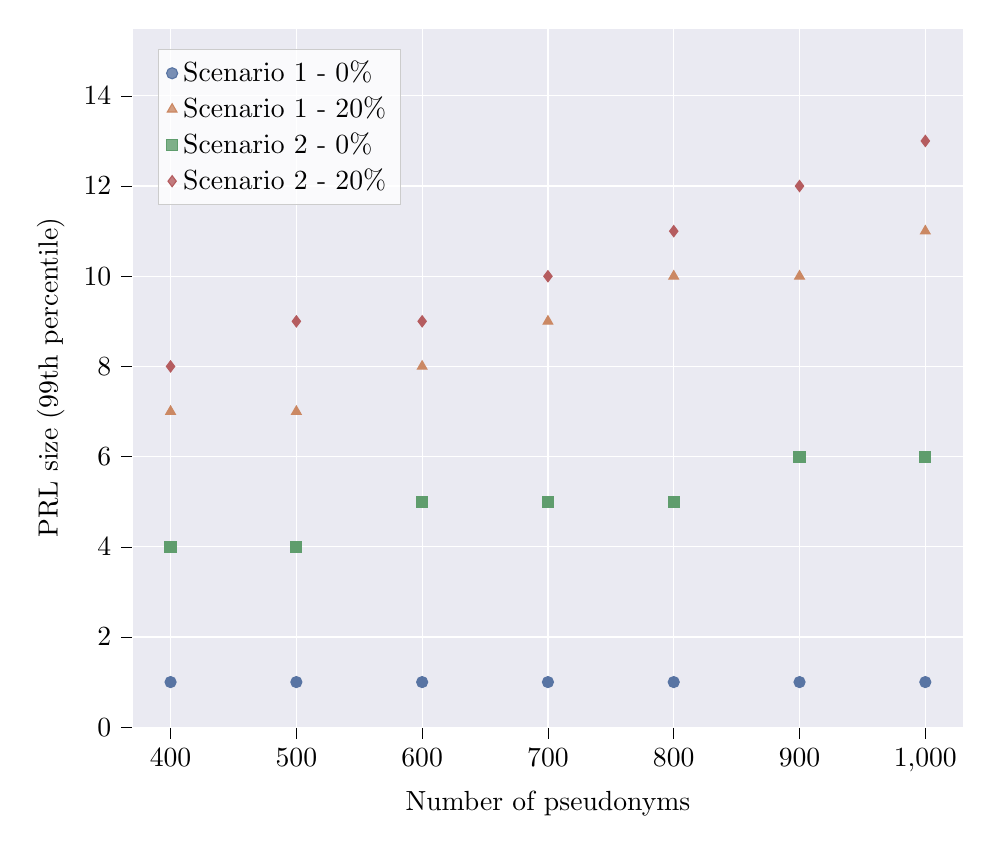
\begin{tikzpicture}

\definecolor{lightgray204}{RGB}{204,204,204}
\definecolor{darkslategray38}{RGB}{38,38,38}
\definecolor{darkslategray76}{RGB}{76,76,76}
\definecolor{indianred1819295}{RGB}{181,92,95}
\definecolor{lavender234234242}{RGB}{234,234,242}
\definecolor{lightslategray133122170}{RGB}{133,122,170}
\definecolor{mediumseagreen95157109}{RGB}{95,157,109}
\definecolor{peru20313699}{RGB}{203,136,99}
\definecolor{steelblue76114176}{RGB}{76,114,176}
\definecolor{steelblue88116163}{RGB}{88,116,163}


\begin{axis}[
width=\columnwidth,
legend pos=north west,
ylabel= PRL size (99th percentile),
xlabel= Number of pseudonyms,
xmajorgrids,
xmajorticks=true,
ymajorgrids,
ymajorticks=true,
axis background/.style={fill=lavender234234242},
axis line style={white},
x grid style={white},
y grid style={white},
legend cell align={left},
legend style={
fill opacity=0.8,
draw opacity=1,
text opacity=1,
at={(0.03,0.97)},
anchor=north west,
draw=lightgray204,
% fill=lavender234234242
},
tick align=outside,
tick pos=left,
xmin=370, xmax=1030,
xtick style={color=black},
ymin=0.0, ymax=15.5,
ytick style={color=black}
]
\addplot [draw=steelblue88116163, fill=steelblue88116163, mark=*, only marks]
table
\addplot [draw=peru20313699, fill=peru20313699, mark=triangle*, only marks]
table
\addplot [draw=mediumseagreen95157109, fill=mediumseagreen95157109, mark=square*, only marks]
table
\addplot [draw=indianred1819295, fill=indianred1819295, mark=diamond*, only marks]
table
\end{axis}

\end{tikzpicture}} 
    \caption{99th percentile PRL sizes for fixed $T_{prl}=30$ and varying number of pseudonyms ($n$) under four scenarios.}
    \label{fig:appendix:markov-n}   
\end{figure}

\begin{figure}[t]
    \centering
    \resizebox{.83\linewidth}{!}{% changed from auto generated plot:
% width=\columnwidth,
% legend pos=north west,
% and escape the % signs in the labels
% Color order: steelblue88116163 peru20313699 mediumseagreen95157109 indianred1819295

% This file was created with tikzplotlib v0.10.1.
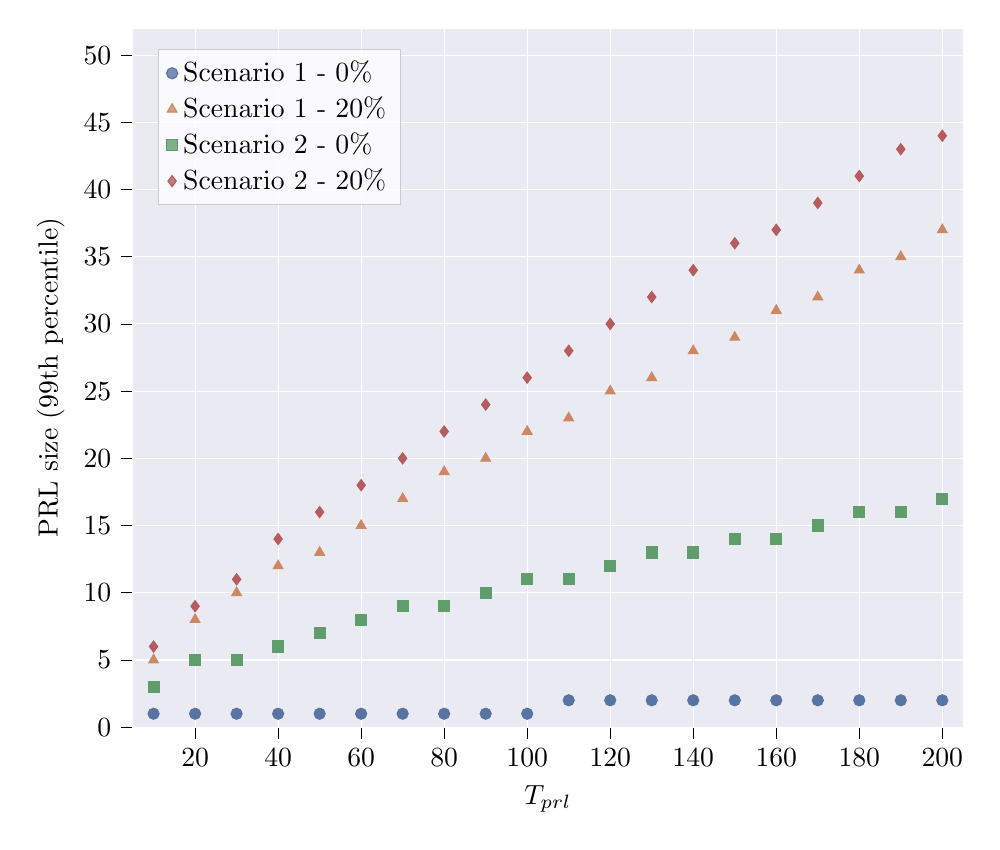
\begin{tikzpicture}

\definecolor{lightgray204}{RGB}{204,204,204}
\definecolor{darkslategray38}{RGB}{38,38,38}
\definecolor{darkslategray76}{RGB}{76,76,76}
\definecolor{indianred1819295}{RGB}{181,92,95}
\definecolor{lavender234234242}{RGB}{234,234,242}
\definecolor{lightslategray133122170}{RGB}{133,122,170}
\definecolor{mediumseagreen95157109}{RGB}{95,157,109}
\definecolor{peru20313699}{RGB}{203,136,99}
\definecolor{steelblue76114176}{RGB}{76,114,176}
\definecolor{steelblue88116163}{RGB}{88,116,163}

\begin{axis}[
width=\columnwidth,
legend pos=north west,
ylabel= PRL size (99th percentile),
xlabel= $T_{prl}$,
xmajorgrids,
xmajorticks=true,
ymajorgrids,
ymajorticks=true,
axis background/.style={fill=lavender234234242},
axis line style={white},
x grid style={white},
y grid style={white},
legend cell align={left},
legend style={
fill opacity=0.8,
draw opacity=1,
text opacity=1,
at={(0.03,0.97)},
anchor=north west,
draw=lightgray204
},
tick align=outside,
tick pos=left,
x grid style={white},
xmin=5, xmax=205,
xtick style={color=black},
y grid style={white},
ymin=0.0, ymax=52,
ytick style={color=black}
]
\addplot [draw=steelblue88116163, fill=steelblue88116163, mark=*, only marks]
table
\addplot [draw=peru20313699, fill=peru20313699, mark=triangle*, only marks]
table
\addplot [draw=mediumseagreen95157109, fill=mediumseagreen95157109, mark=square*, only marks]
table
\addplot [draw=indianred1819295, fill=indianred1819295, mark=diamond*, only marks]
table
\end{axis}

\end{tikzpicture}
} 
    \caption{99th percentile PRL sizes for fixed $n=800$ pseudonyms and varying $T_{prl}$ under four scenarios.}
    \label{fig:appendix:markov-e}  
\end{figure}

In the following, we expand this evaluation with Figures
\ref{fig:appendix:markov-n} and \ref{fig:appendix:markov-e}.
\Cref{fig:appendix:markov-n} depicts only the 99th percentile for a fixed
$T_{prl}$ and only focuses on the four extreme cases: For each of the two
baseline scenarios, 0\% and 20\% of attackers in the network. The horizontal
axis then depicts a growing number of pseudonyms (and, therefore, vehicles) in
the network. This is to show that a larger number of vehicles does not
exponentially grow the expected size of the \ac{PRL}. Instead, the 99th
percentile of the list size grows linearly with $n$. Similarly,
\cref{fig:appendix:markov-e} shows the same situation for a fixed number of
pseudonyms at $n=800$ but a varying window for $T_{prl}$. This second graph
shows that the \ac{PRL} size also grows linearly with a linear increase in the
time that a pseudonym stays in the \ac{PRL}.

\subsection{Probabilities and Expected Revocations}

Above, $p$ is the probability of revocation in each time step. As time steps are at the granularity of seconds, and our system runs for a long time, it turns out that the per-step probabilities leading to realistic revocation rates are very small. Instead, the probabilities used in the \ac{PRL} size evaluation were described in terms of a compound probability $q$ that a revocation occurs at least once over a number of $s$ steps. This probability can be computed via the geometric series
\[q(p,s) = \sum_{i=1}^s p\cdot(1-p)^{i-1} = 1-(1-p)^s\] 
which sums up the probabilities that the first revocation occurs the first time in step $i\in[1:s]$. Note that this is equal to $1$ minus the probability that in all $s$ steps no revocation occurs. Solving for $p$ we obtain
\[p(q,s) = 1-\sqrt[s]{1-q}\,.\]
We used this formula to compute the baseline per-step probabilities underlying our scenarios for honest vehicle and attacker separately. The final probabilities $p$ for the Markov models were then obtained by averaging the probabilities weighted according to the share of attackers.

For estimating the expected numbers of revocations in our scenarios we needed to calculate the expected value for $n$ pseudonyms over $s$ steps. If each step was independent this would simply be $n\cdot s \cdot p$, however, as explained above, in our Markov model at most $n$ pseudonyms can be revoked at a time. We compensated for this fact by taking into account the chance $p_{\mathrm{prl}}$ that a given pseudonym is on the \ac{PRL} at any given time and computed the desired estimate $E_{\mathrm{rev}}$:
\[ E_{\mathrm{rev}}=n\cdot s \cdot p \cdot (1-p_{\mathrm{prl}}) \]
We set $p_{\mathrm{prl}}$ to the median \ac{PRL} size, as obtained by the Markov model for each scenario, divided by $n$.
